\documentclass[AMA,STIX1COL,]{WileyNJD-v2}



% tightlist command for lists without linebreak
\providecommand{\tightlist}{%
  \setlength{\itemsep}{0pt}\setlength{\parskip}{0pt}}



\usepackage{longtable}
\newcommand{\srb}[1]{\textsf{\textcolor{red}{#1}}}
\usepackage{ulem}
\usepackage{placeins}
\newcommand{\sigmoid}{\mathrm{sigmoid}}
\renewcommand{\thefootnote}{\alph{footnote}}

\articletype{Research article}

\received{2022-04-29}

\revised{2022-06-01}

\accepted{2022-07-01}

\raggedbottom

\begin{document}


\title{Case-Base Neural Networks: survival analysis with time-varying,
higher-order interactions}

\author[a]{Jesse Islam}
\author[b]{Maxime Turgeon}
\author[c]{Robert Sladek}
\author[d]{Sahir Bhatnagar}

\authormark{Islam \emph{et al}.}

\address[a]{Department of Quantitative life sciences, McGill University}
\address[b]{Department of Statistics, University of Manitoba}
\address[c]{Department of Human Genetics, McGill University}
\address[d]{Department of Biostatistics, McGill University}

\corres{\email{jesse.islam@mail.mcgill.ca}}


\abstract{In survival analysis, covariate interactions are difficult to
model without prior knowledge using regression-based methods. Neural
network-based survival models have been developed for data-driven
interaction modeling, however, these approaches lack implementations for
time-varying interactions or a flexible baseline hazard. To address
this, we extend the case-base sampling framework and propose Case-Base
Neural Networks (CBNN), which introduce time directly into the model,
using commonly available neural network components for a simple
implementation. First, we case-base sample the survival data, converting
the survival time of each participant into discrete moments in time.
This allows us to estimate the probability an event occurs at a given
moment using a neural network to get the hazard. We compare CBNN to
survival methods based on regression and neural networks in two
simulations and two real data applications with a fixed neural network
architecture. We report metrics for each model over follow-up time using
both a proper (Index of Prediction Accuracy) and non-proper (inverse
probability censoring weights-adjusted concordance index) scoring rule.
A simple simulation shows CBNN outperforming the other neural network
methods. The complex simulation highlights the ability of CBNN to model
both a complex baseline hazard and time-varying interactions,
outperforming all competitors. The first real data application shows
CBNN outperforming all neural network competitors, while a second real
data application shows competitive performance. CBNN has shown that it
is more consistent in prediction performance across time in the
simulations and real data applications compared to the competing neural
network approaches.}

\keywords{survival analysis, machine learning, case-base, neural
network}

\maketitle

\hypertarget{introduction}{%
\section{Introduction}\label{introduction}}

The widespread use of the Cox proportional hazards model has led to a
focus on survival models based on hazard ratios and relative risks
rather than on survival curves and absolute risks \citep{hanley2009}. In
clinical settings, Cox models are frequently prioritized over
smooth-in-time accelerated failure time (AFT) models \citep{hanley2009},
which can estimate absolute risks by modeling the hazard directly
through user specification of a baseline hazard distribution. The user
may forgo this choice by implementing a flexible set of parameters using
splines, as proposed by Royston and Palmar \citep{royston2002flexible}.
These regression models also require user-specified interactions, which
may limit risk prediction accuracy.

Over longer follow-up, it is challenging to maintain the proportional
hazards assumption as the risk associated with each covariate may not be
constant with time. Previous studies related to breast cancer have
discovered time-varying interactions with covariates of interest, like
tumor size \citep{coradini2000time} \citep{hilsenbeck1998time}. Another
limitation of regression-based models is the requirement of prior
knowledge; the analyst must know potential time-varying interactions and
explicitly evaluate them.

Data-driven neural network approaches bypass the need for prior
knowledge of interaction terms. DeepSurv is a semi-parametric
proportional hazards neural network model that implements the Cox
partial log-likelihood as a custom loss function
\citep{katzman2018DeepSurv}. This results in a stepwise absolute risk
curve that cannot accommodate time-varying interactions. Compared to Cox
regression, DeepSurv has shown a small improvement in performance using
a single layer neural network on the Study to Understand Prognoses
Preferences and Risk Treatments (SUPPORT) dataset
\citep{knaus1995SUPPORT}. Farraggi et al.~suggested a modification to
the loss function required for a Cox neural network that can model
non-proportional hazards \citep{faraggi1995neural}. Wang et al.~took the
concept of extreme learning machines and applied them in a survival
context, removing the need for tuning the number of layers and nodes
\citep{wang2019extreme}. A Cox-based neural network combined with Local
Interpretable Model-Agnostic Explanations (LIME)
\citep{ribeiro2016model} interprets the association of each Single
Nucleotide Polymorphism (SNP) \citep{sun2020genome} to a phenotype.

DeepHit requires each survival time of interest to be specified in the
model and directly estimates survival curves, rather than deriving a
hazard function \citep{lee2018DeepHit}. It assumes an inverse Gaussian
distribution as the baseline hazard and its concordance index (c-index)
score outperforms DeepSurv \citep{katzman2018DeepSurv} on the Molecular
Taxonomy of Breast Cancer International Consortium (METABRIC) dataset
\citep{curtis2012genomic}.

Ripley et al.~presented seven different distributions and modeling
paradigms based on neural networks \citep{ripley2004non}. They provided
the methodology behind parametric log-logistic and log-normal neural
network models. Like DeepHit, these models are restricted to one of the
seven baseline hazard distributions, reducing the flexibility of the
average survival prediction.

Deep Survival Machines (DSM) provides a flexible, parametric survival
model using neural networks with a mixture of distributions as the
baseline hazard \citep{dsmPaper}. DSM allows the user to specify a
mixture of distributions for a flexible baseline hazard. On both the
SUPPORT and METABRIC datasets, DSM outperforms DeepSurv and DeepHit
\citep{dsmPaper}. However, like DeepHit and DeepSurv, DSM cannot model
time-varying interactions.

These methods need custom loss and activation functions that are
difficult to implement in practice. We note the complexity of these
alternative neural network approaches; DeepSurv, DeepHit, and DSM all
require custom loss functions \citep{katzman2018DeepSurv}
\citep{lee2018DeepHit} \citep{dsmPaper}, while DSM requires user
implementations for distributions beyond Log-Normal or Weibull and a
two-phase learning process \citep{dsmPaper}. Regression-based approaches
require prior specification of all interaction terms, which makes it
challenging to model covariate effects that change over time. In this
article, we propose Case-Base Neural Networks (CBNN) as a method that
models time-varying interactions and a flexible baseline hazard using
commonly available neural network components. Our approach to modeling
the full hazard uses case-base sampling \citep{hanley2009}, which allows
probabilistic models to predict survival outcomes. Following the
case-base framework, we can use transformations of time as a feature
(covariate) to specify different baseline hazards. For example, by
including splines of time as covariates, we can approximate the
Royston-Parmar flexible baseline hazard model
\citep{royston2002flexible}. An alternative approach to Royston-Parmar
is case-base with logistic regression (CBLR), which provides some
flexibility in modeling, but still requires user specification of
time-varying interactions and baseline hazard, while CBNN can model both
without user specification; only a sufficiently deep network is
required.

In Section \ref{methods}, we describe how case-base sampling and neural
networks are combined both conceptually and algebraically, along with
our hyperparameter choice and software implementation. Then, in Section
\ref{sims}, we describe our metrics and compare the performance of CBNN,
DeepSurv, DeepHit, DSM, Cox regression, and case-base using logistic
regression on simulated data. Next, Section \ref{casestudies} describes
the real-data analysis, while in Section \ref{discussion}, we explore
the implications of our results and contextualize them within neural
network survival analysis in a single event setting.

\hypertarget{methods}{%
\section{Case-base neural network methodology, metrics, and
software}\label{methods}}

In this section, we define case-base sampling, which converts the total
survival time into discrete person-specific moments (person-moments).
Then, we detail how neural networks can be used within this framework,
explicitly incorporating time as a feature while adjusting for the
sampling bias. Finally, we report on the software versions used. A
package is available for use at {[}GITHUBLINK{]}. The entire code base
to generate the analyses in this paper is available at {[}GITHUB
LINK{]}.

\hypertarget{case-base-sampling}{%
\subsection{Case-base sampling}\label{case-base-sampling}}

Case-base sampling is an alternative framework for survival analysis
\citep{hanley2009}. In case-base sampling, we sample from the continuous
survival time of each person in our dataset to create a \emph{base
series} of \emph{person-moments}. This \emph{base series} complements
the \emph{case series}, which contains all person-moments at which the
event of interest occurs.

For each person-moment sampled, let \(X_i\) be the corresponding
covariate profile \(\left(x_{i1},x_{i2},...,x_{ip} \right)\), \(T_i\) be
the time of the person-moment, and \(Y_i\) be the indicator variable for
whether the event of interest occurred at time \(T_i\). We estimate the
hazard function \(h(t \mid X_i)\) using the sampled person-moments.
Recall that \(h(t \mid X_i)\) is the instantaneous potential of
experiencing the event at time \(t\) for a given set of covariates
\(X_i\), assuming \(T_i \geq t\).

Now, let \(b\) be the (user-defined) size of the \emph{base series}, and
let \(B\) be the sum of all follow-up times for the individuals in the
study. If we sample the \emph{base series} uniformly, then the hazard
function of the sampling process is equal to \(b/B\). Therefore, we have
the following equality
\footnote{We are abusing notation here, conflating hazards with probabilities. For a rigorous treatment, see Saarela \& Hanley (2015) section 3 \cite{saarela2015} .}:
\begin{align}\label{eqn:main}
\frac{P\left(Y_i=1 \mid X_i, T_i\right)}{P\left(Y_i = 0 \mid X_i, T_i\right)} = \frac{h\left(T_i \mid X_i\right)}{b/B}.
\end{align} The odds of a person-moment being a part of the \emph{case
series} is the ratio of the hazard \(h(T_i \mid X_i)\) and the uniform
rate \(b/B\). Using \eqref{eqn:main}, we can see how the log-hazard
function can be estimated from the log-odds arising from case-base
sampling: \begin{align}\label{eqn:offset}
\log \left( h\left(t \mid X_i\right)\right) = \log \left(\frac{P\left(Y_i = 1 \mid X_i, t\right)}{P\left(Y_i = 0 \mid X_i, t\right)}\right) + \log\left(\frac{b}{B}\right).
\end{align}

We may estimate the hazard function if we adjust for the bias introduced
when sampling a fraction of the study base \(B\) by adding the offset
term \(\log\left(\frac{b}{B} \right)\) (\eqref{eqn:offset}). Next, we
propose using neural networks to model the odds.

\hypertarget{neural-networks-to-model-the-hazard-function}{%
\subsection{Neural networks to model the hazard
function}\label{neural-networks-to-model-the-hazard-function}}

After case-base sampling, we pass all features, including time, into any
user-defined feed-forward component, to which an offset term (to adjust
for bias from case-base sampling) is added, then passed through a
sigmoid activation function (Figure \ref{fig:NNarch}). We use the
sigmoid function as its inverse is the odds, which we can use to
calculate the hazard. The general form for the neural network using CBNN
is:

\begin{align}\label{eqn:nnProb}
P\left(Y=1|X,T\right)&=\mathrm{sigmoid}\left(f_{\theta}(X, T) + \log\left(\frac{B}{b}\right) \right),
\end{align}

where \(T\) is a random variable representing the event time, \(X\) is
the random variable for a covariate profile, \(f_{\theta}(X, T)\)
represents any feed-forward neural network architecture,
\(\log\left(\frac{B}{b}\right)\) is bias term set by case-base sampling,
\(\theta\) is the set of parameters learned by the neural network and
\(\mathrm{sigmoid}(x)=\frac{1}{1+e^{-x}}\). By allowing a neural network
to approximate a higher-order polynomial of time, the baseline hazard
specification is now data-driven, where user-defined hyperparameters
such as regularization, number of nodes, and layers control the
flexibility of the model. We provide a detailed description of the
choices we made in the next sub-section.

\begin{figure}

{\centering 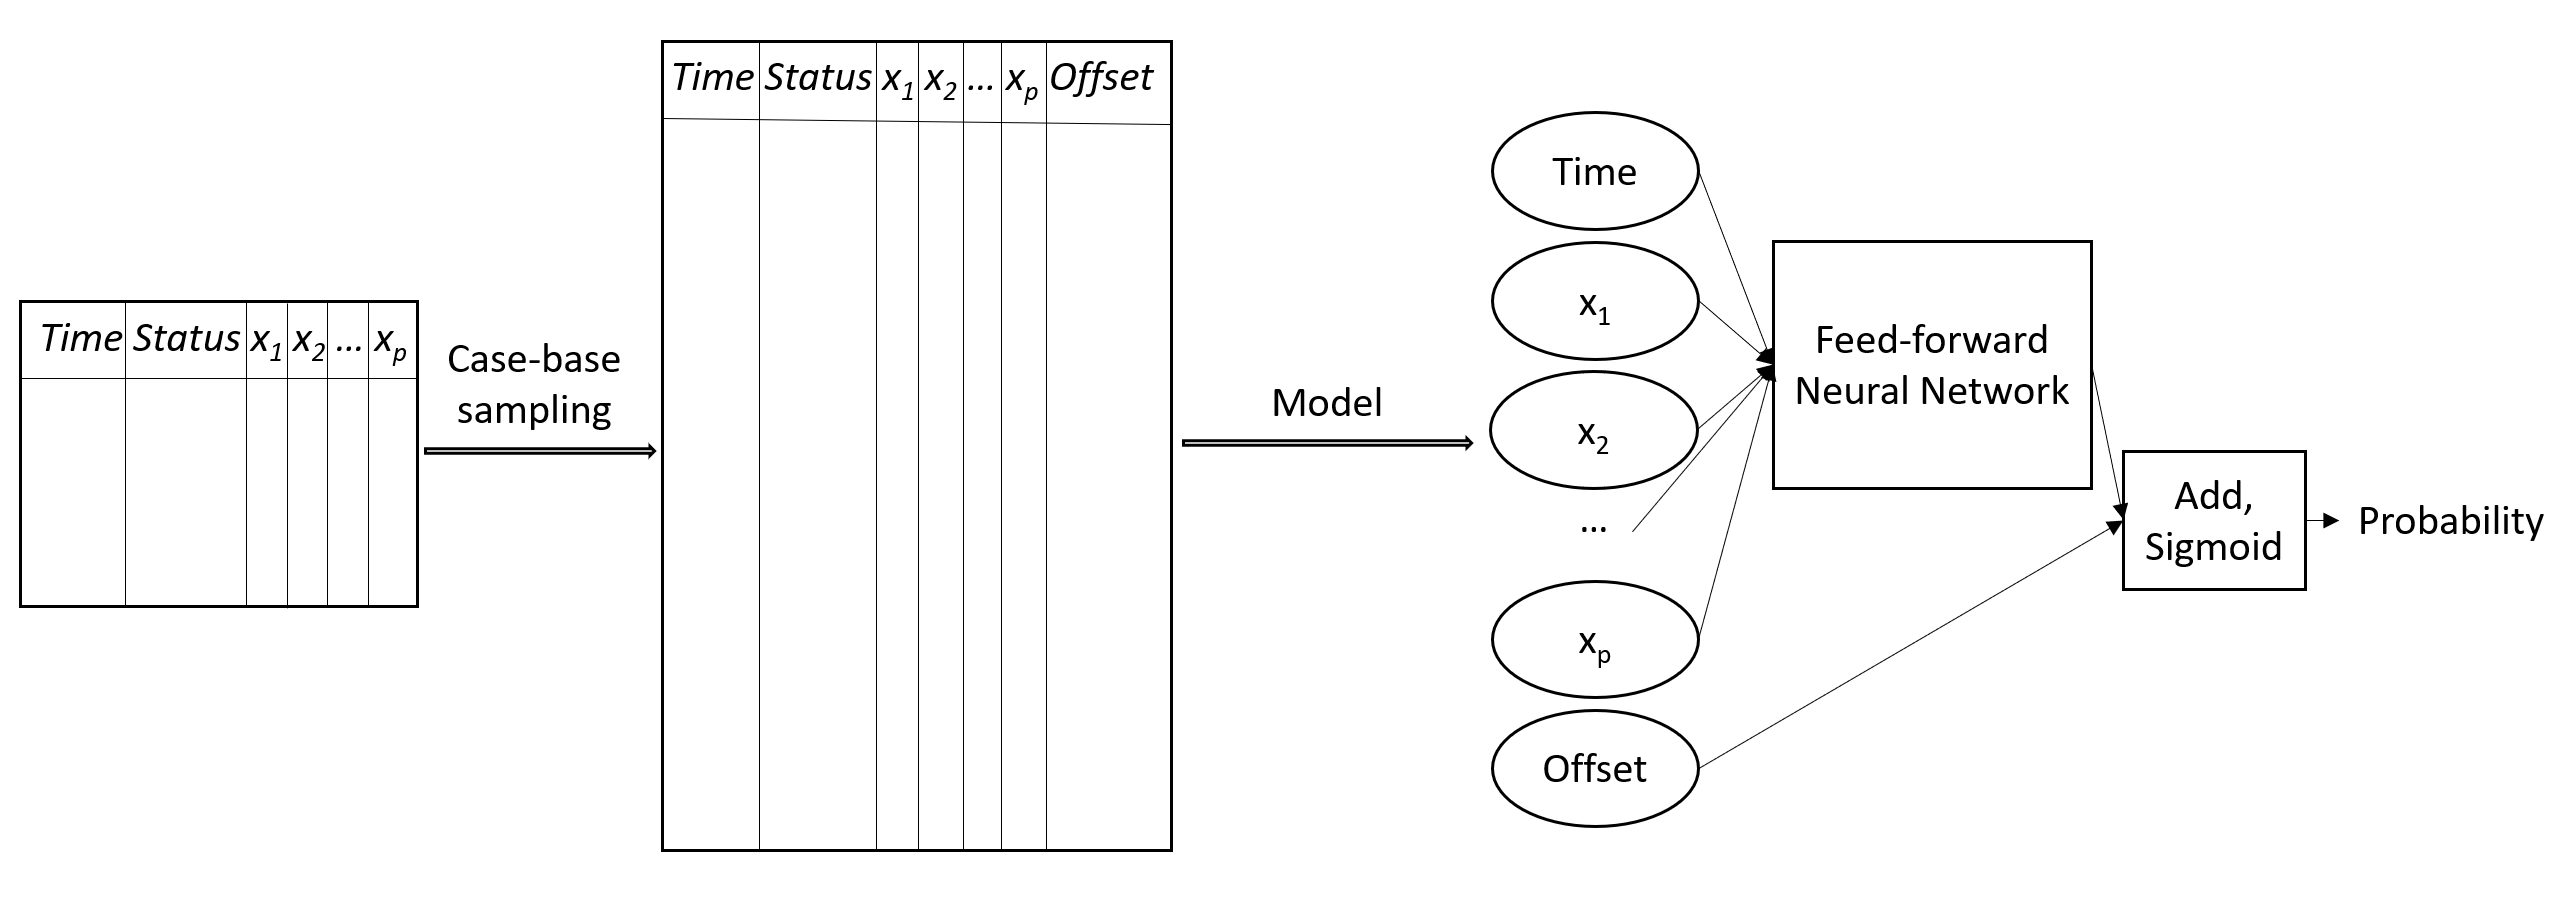
\includegraphics[width=1\linewidth]{/home/bhatnagar-lab/jislam/pmnnProjects/paper/figures/nnarch2} 

}

\caption{Steps involved in CBNN from case-base sampling to the model framework we use for training. The first step is case-base sampling, completed before training begins. Next, we pass this sampled data through a feed-forward neural network. We add the offset and pass that through a sigmoid activation function, whose output is a probability. Once the neural network model completes its training, we can convert the probability output to a hazard, using it for our survival outcomes of interest.}\label{fig:NNarch}
\end{figure}

The following derivation shows how our probability estimate is converted
to odds: \begin{align*}
 \log\left( h(t \mid X_i) \right) &= \log\left(\frac{\mathrm{sigmoid}\left(f_{\theta}(X, T) + \log\left(\frac{B}{b}\right)\right)}{1-\mathrm{sigmoid}\left(f_{\theta}(X, T) + \log\left(\frac{B}{b}\right)\right)}\right) + \log\left(\frac{b}{B}\right) \\
 &= \log\left( \frac{\frac{\exp\left(f_{\theta}(X, T) + \log\left(\frac{B}{b}\right)\right)}{\exp\left(f_{\theta}(X, T) + \log\left(\frac{B}{b}\right)\right)+1}}{1-\frac{\exp\left(f_{\theta}(X, T) + \log\left(\frac{B}{b}\right)\right)}{\exp\left(f_{\theta}(X, T) + \log\left(\frac{B}{b}\right)\right)+1}}\right) + \log\left(\frac{b}{B}\right) \\
 &= \log\left(\exp\left( f_{\theta}(X, T) + \log\left(\frac{B}{b}\right) \right) \right) + \log\left(\frac{b}{B}\right) \\
 &= f_{\theta}(X, T) + \log\left(\frac{B}{b}\right) + \log\left(\frac{b}{B}\right) \\
&= f_{\theta}(X, T). 
\end{align*}

We use binary cross-entropy as our loss function \citep{gulli2017}:
\begin{align*}
L(\theta)=-\frac{1}{N} \sum^{N}_{i=1} y_{i} \cdot \log(\hat{f}_{\theta}(x_{i}, t_{i}) ) + (1-y_{i} )\cdot \log(1-\hat{f}_{\theta}(x_{i}, t_{i}) ),
\end{align*} where \(\hat{f}_{\theta}(x_{i}, t_{i})\) is our estimate
for a given covariate profile and time, \(y_{i}\) is our target value
specifying whether an event occurred, and \(N\) represents the number of
individuals in our training set.

Backpropagation is used to optimize the parameters in the model with an
appropriate minimization algorithm (e.g.~Adam, RMSPropagation,
stochastic gradient descent)\citep{gulli2017}. For our analysis, we use
Adam. Note that the size of the \emph{case series} is fixed as the
number of events, but we can make the \emph{base series} as large as we
want. A ratio of 100:1 \emph{base series} to \emph{case series} is
sufficient \citep{hanley2009}. We pass our feed-forward neural network
through a sigmoid activation function (Figure \ref{fig:NNarch}).
Finally, we can convert this model output to a hazard. When using our
model for predictions, we manually set the offset term to 0 in the new
data, as we account for the bias during the fitting process.

Since we are directly modeling the hazard, we can readily estimate the
risk function (\(F\)) at time \(t\) for a covariate profile \(X\),
viz.\begin{align}\label{eqn:ci2}
F\left(t|X\right)& = 1 - \exp\left(-\int_{0}^{t}h(u|X) \,\textrm du\right).
\end{align} We use Riemann's Sum \citep{hughes2020calculus} to
approximate the integral in \eqref{eqn:ci2}.

\hypertarget{hyperparameter-selection}{%
\subsection{Hyperparameter selection}\label{hyperparameter-selection}}

Neural networks provide flexibility when defining the architecture and
optimization parameters of our models. These hyperparameter choices can
affect the estimated parameters and were chosen during a set of initial
simulations to determine if CBNN can learn complex interactions in
practice. We set a max number of epochs to be \(2000\), batch size as
\(512\), learning rate as \(10^{-3}\), decay as \(10^{-7}\), patience as
\(10\) epochs, \(\{50,50,25,25\}\) nodes in each hidden layer with
\(50\%\) dropout at each layer, a validation split of \(20\%\), a
testing split of \(10%
\), a minimum delta loss on the validation set of \(10^{-7}\) over 10
epochs, and Adam \citep{gulli2017} as our optimizer. These choices may
permit the model to approximate higher-order interactions while
preventing over-fitting \citep{srivastava2014dropout}. We fix a
train-validation-test split that allows us to update the weights with a
subset of the data (training), assess performance at each epoch
(validation) and gauge performance of the final model (test). We select
the best weights after training based on validation loss
\citep{gulli2017}.

\hypertarget{software-implementation}{%
\subsection{Software implementation}\label{software-implementation}}

R \citep{Rsoft} and python \citep{py} are used to evaluate methods from
both languages. We fit the Cox model using the \textbf{survival} package
\citep{survpkg}, the CBLR model using the \textbf{casebase} package
\citep{cbpkg}, the DeepSurv model using the \textbf{survivalmodels}
package \citep{survmods}, the DSM model using
\textbf{DeepSurvivalMachines} \citep{dsmPaper} and the DeepHit model
using \textbf{pycox} \citep{lee2018DeepHit}. We made the components of
CBNN using the \textbf{keras} \citep{keras} package and the
\textbf{casebase} package for the sampling step. The \textbf{simsurv}
package \citep{simsurv} is used to simulate our simulation studies,
while \textbf{flexsurv} \citep{flexsurv} is used to fit a flexible
baseline hazard using splines for our complex simulation. We use the
implementation of c-ipcw from the python package \textbf{sksurv}
\citep{sksurv}. The \textbf{riskRegression} package
\citep{riskRegression} is used to get the Brier score and IPA metrics.
We changed the \textbf{riskRegression} package to be used with any user
supplied risk function \(F\). To ensure that both R and Python-based
models are running in unison on the same data through our simulations
and bootstrap, we use the \textbf{reticulate} package
\citep{reticulate}.

\hypertarget{sims}{%
\section{Simulation studies}\label{sims}}

In this section, we use simulated data to evaluate the performance of
CBNN and compare our approach with existing methods based on regression
(Cox, CBLR) and neural network (DeepHit, DeepSurv, DSM) methods. We
specify a linear combination of each covariate as the linear predictor
in regression-based approaches (Cox, CBLR), which contrasts with neural
network approaches that allow for non-linear interactions. We simulate
data under a simple exponential model, and a complex baseline hazard
with time-varying interactions, each with 10\% random censoring. For
both settings, we simulate three covariates:

\[
z_{1} \sim \textrm{Bernoulli}(0.5) \qquad \qquad
z_{2} \sim \begin{cases}
 N(0,0.5) & \textrm{if } z_{1}=0\\ 
 N(10,0.5) & \textrm{if } z_{1}=1
\end{cases} \qquad \qquad
z_{3} \sim \begin{cases}
 N(8,0.5) & \textrm{if } z_{1}=0\\ 
 N(-3,0.5) & \textrm{if } z_{1}=1.
\end{cases}
\]

The DeepHit-specific hyperparameter alpha is set to \(0.5\) (equal
weight between its negative log-likelihood and ranking losses
\citep{lee2018DeepHit}). We change the \textbf{DeepSurvivalMachines}
\citep{dsmPaper} package to include dropout and a minimum delta loss
during the fitting process. For DSM, we define a mixture model of six
Weibull distributions for the baseline hazard. All other hyperparameters
are held constant across all neural network methods in both the
simulation studies and real data applications.

Besides the methods mentioned above, we include the Optimal model in our
comparisons using CBLR. That is, we include the exact functional form of
the covariates in a CBLR model (referred to as Optimal for simplicity).
We calculate \(t\)-based 95\% confidence intervals using 100
replications of the simulated data For all analyses, we use 80\% for
training and 20\% for the test set. 20\% of the training set is kept for
validation at each epoch. We predict risk functions \(F\) using
\eqref{eqn:ci2} for individuals in the test set, which are used to
calculate our c-ipcw and IPA scores.

\hypertarget{performance-metrics}{%
\subsection{Performance metrics}\label{performance-metrics}}

We use two metrics to assess the performance of the different methods of
interest: 1) index of prediction accuracy (IPA) \citep{kattan2018index}
and 2) inverse probability censoring weights-adjusted concordance index
(c-ipcw) \citep{uno2011}, which we define below. Both these
time-dependent metrics provide transparency as to when in follow-up time
each model may perform better than the others.

\hypertarget{index-of-prediction-accuracy-ipa}{%
\subsubsection{Index of prediction accuracy
(IPA)}\label{index-of-prediction-accuracy-ipa}}

The IPA is a function of the Brier score (\(BS(t)\)) \citep{graf1999},
which is defined as \begin{align}
BS(t)=\frac{1}{N}\sum^{N}_{i=1}\left(\frac{\left(\widehat{F}(X_{i},t)-1\right)^{2}\cdot I_{T_{i}\leq t,\delta_{i}=1}}{\widehat{G}(T_{i})} + \frac{\left(\widehat{F}(X_{i},t)\right)^{2}\cdot I_{T_{i}>t}}{\widehat{G}(t)}\right),
\end{align} where \(\delta_{i}=1\) shows individuals who have
experienced the event, \(N\) represents the number of samples in our
dataset over which we calculate \(BS(t)\), \(\widehat{G}(t)=P[C>t]\) is
a non-parametric estimate of the censoring distribution, \(C\) is
censoring time and \(T_{i}\) is an individual's survival or censoring
time. The Brier score provides a score that accounts for the information
loss because of censoring. There are three categories of individuals
that may appear within the dataset once we fix our \(t\) of interest.
Individuals who experienced the event before \(t\) are present in the
first term of the equation. The second term of the equation includes
individuals who experience the event or are censored after \(t\). Those
censored before \(t\) are the third category of people. The inverse
probability censoring weights (IPCW) adjustment (\(G(\cdot)\)) is to
account for these category three individuals whose information is
missing. The IPA score as a function of time is given by \begin{align}
\textrm{IPA}(t) &= 1-\frac{BS_{model}(t)}{BS_{null}(t)}, \nonumber
\end{align} where \(BS_{model}(t)\) represents the Brier score over time
\(t\) for the model of interest, and \(BS_{null}(t)\) represents the
Brier score if we use an unadjusted Kaplan-Meier curve as the prediction
for all observations \citep{kattan2018index}. Note that IPA has an upper
bound of one, where positive values show an increase in performance over
the null model and negative values show that the null model performs
better. These scores demonstrate how performance changes over follow-up
time.

A potential artifact of IPA is that the score is unstable at earlier and
later survival times. This is because of a near equivalent Brier score
between each model and the null model. At small values, a difference of
\(0.1\) creates a more significant fold change than at larger values. As
the Brier score is potentially small at the start and at the end of
their respective curves, we may see instability of the IPA score at
those ends.

\hypertarget{inverse-probability-censoring-weights-adjusted-concordance-index}{%
\subsubsection{Inverse probability censoring weights-adjusted
concordance
index}\label{inverse-probability-censoring-weights-adjusted-concordance-index}}

The c-ipcw is a non-proper, rank-based metric that does not depend on
the censoring times in the test data \citep{uno2011}. The c-ipcw is
given by

\begin{align} \label{eq:cidx}
c-ipcw(t) &= \frac{\sum^{N}_{i=1}\sum^{N}_{j=1}\delta_{i}\left\{\widehat{G}(T_{i})\right\}^{-2} I(T_{i}<T_{j},T_{i}<t) I\left(\widehat{F}(t|X_{i})>\widehat{F}(t|X_{j})\right)}{\sum^{N}_{i=1}\sum^{N}_{j=1}\delta_{i}\left\{\widehat{G}(T_{i})\right\}^{-2} I(T_{i}<T_{j},T_{i}<t)},
\end{align} where the follow-up period of interest is (0,\(t\)),
\(I(\cdot)\) is an indicator function, \(\widehat{F}(X_{i},t)\) is the
risk function estimated for everyone in the study at time \(t\) and
c-ipcw can compare the performance of different models, where a higher
score is better. Note that the c-ipcw may produce misleading
performance, as it ranks based on survival times, not event status
\citep{cindexfails2019}. This metric is considered an unbiased
population concordance measure because of the IPCW adjustment
\citep{uno2011}.

\srb{in figure 2 i changed $C_{IPCW}$ to c-ipcw, as capital C is used for censoring. in the plots, would it make sense to leave it as a small letter?}

\begin{figure}

{\centering 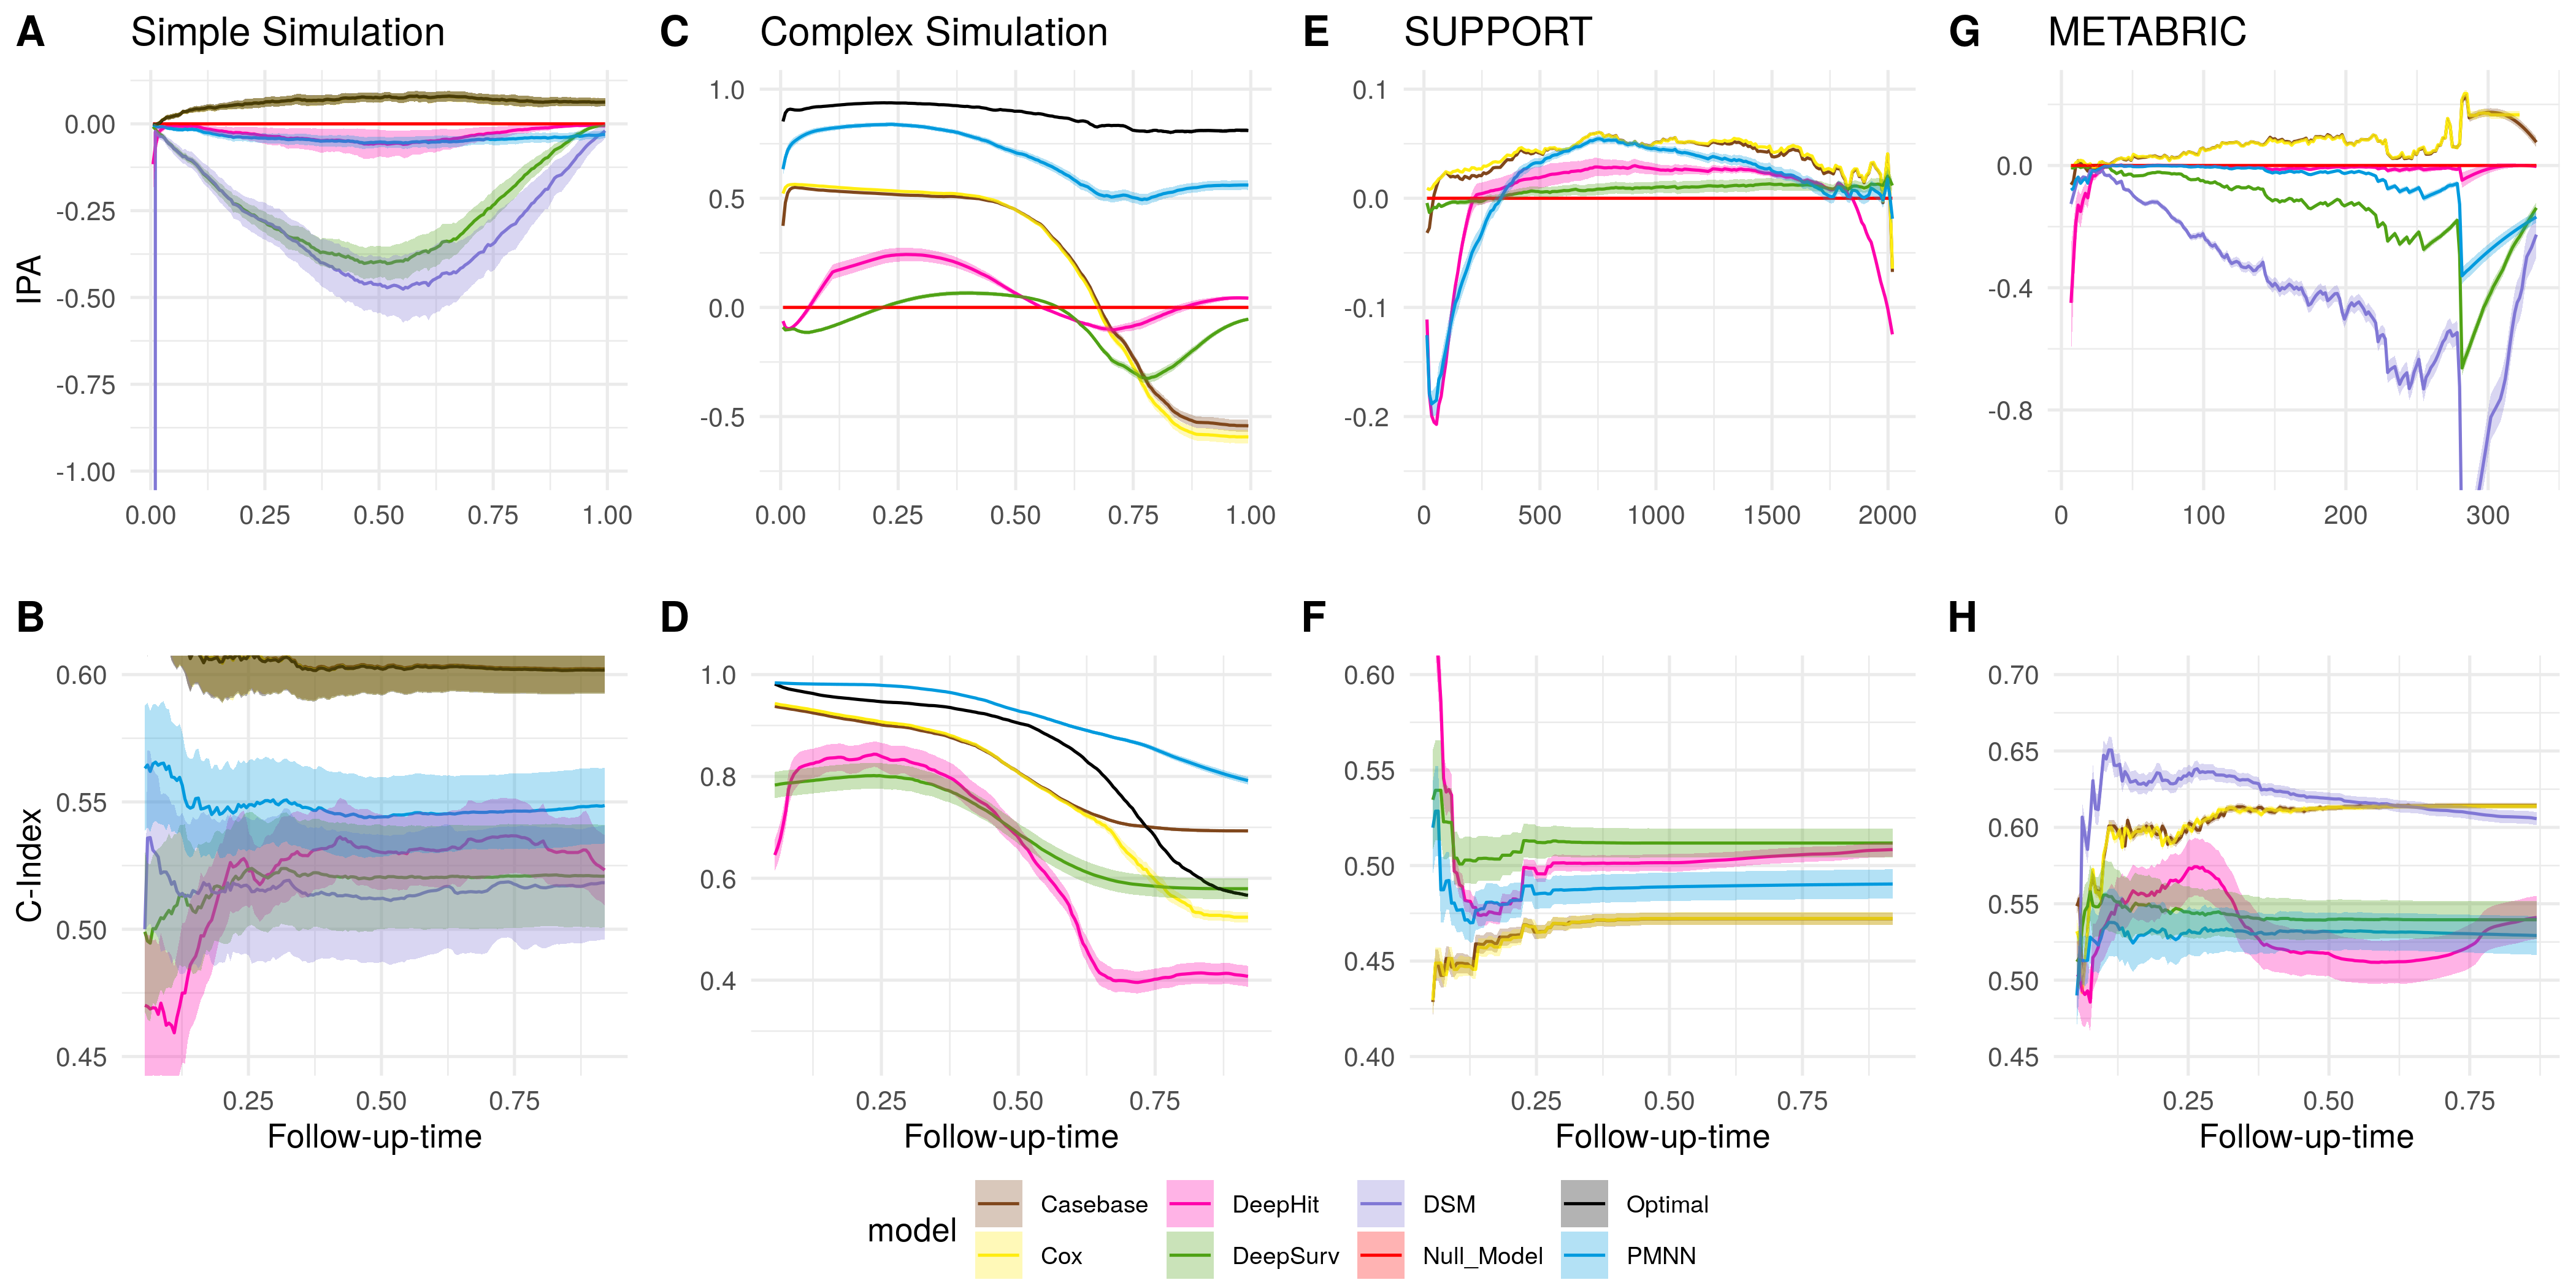
\includegraphics[width=1\linewidth]{/home/bhatnagar-lab/jislam/pmnnProjects/paper/../pmnnPlayground/reviewedAnalysisPMNN/figures/megaPlot} 

}

\caption{Summarizes the simple simulation (A, B), complex simulation (C, D), SUPPORT case study (E, F) and METABRIC case study (G, H) results. The first row shows the IPA score for each model in each study over follow-up time. Negative values mean our model performs worse than the null model and positive values mean the model performs better. The second row shows the c-ipcw for each model in each study over follow-up time. A score of 1 is the maximum performance for either metric. Each model-specific metric in each study shows a 95-percent confidence interval over 100 iterations. The models of interest are case-base with logistic regression (CBLR), Case-Base Neural Networks (CBNN), Cox, DeepHit, DeepSurv, Deep Survival Machines (DSM), Optimal (a CBLR model with the exact interaction terms and baseline hazard specified) and Kaplan-Meier (to serve as a baseline, predicting the average for all individuals).}\label{fig:megaPlot}
\end{figure}

\hypertarget{simple-simulation-constant-baseline-hazard}{%
\subsection{Simple simulation: constant baseline
hazard}\label{simple-simulation-constant-baseline-hazard}}

We simulate data from a simple model that primarily depends on a
constant baseline hazard:
\[h(t \mid X_i) = \lambda\cdot e^{\beta_{{1}}z_{1}+\beta_{{2}}z_{2}+\beta_{{3}}z_{3}},\]
with minimal covariate effects given by
\(\beta_{{1}}=0.1, \beta_{{2}}=0.1, \beta_{{3}}=0.1\) and
\(\lambda=1.0\). Once we simulate survival times, we introduce 10\%
random censoring.

\hypertarget{performance-comparison-in-simple-simulation}{%
\subsubsection{Performance comparison in simple
simulation}\label{performance-comparison-in-simple-simulation}}

Figure \ref{fig:megaPlot} A, B and Table \ref{tab:megaTable} A show the
results for the simple simulation. The regression-based methods (CBLR,
Cox, Optimal) outperform the neural network ones in the simple
simulation setting. Among the neural network approaches, CBNN
outperforms all other methods in terms of both IPA and c-ipcw (Figure
\ref{fig:megaPlot} A, B). Specifically, we see CBNN is consistent across
time with smaller confidence intervals compared to DeepHit, DeepSurv and
DSM.

In this simple setting, the regression models are much closer to the
Optimal model, while the neural network models perform worse than the
null model. The wide confidence bands in c-ipcw suggest the neural
network models may be over-parameterized.

\hypertarget{complex-simulation-flexible-baseline-hazard-time-varying-interactions}{%
\subsection{Complex simulation: flexible baseline hazard, time-varying
interactions}\label{complex-simulation-flexible-baseline-hazard-time-varying-interactions}}

This simulation demonstrates performance with the presence of a complex
baseline hazard and a time-varying interaction. Originally used to
demonstrate the spline-based hazard model proposed by Royston and Parmar
\citep{royston2002flexible}, the breast cancer dataset provides a
complex hazard from which we simulate, available in the
\textbf{flexsurv} R package \citep{flexsurv}. To increase the complexity
of our data-generating mechanism for this simulation, we design the
model as follows: \begin{align}
h(t \mid X_i) =\sum_{i=1}^{5} (\gamma_{i} \cdot \psi_{i}) + \beta_{{1}} (z_{1}) + \beta_{{2}} (z_{2})+ \beta_{{3}} (z_{3})+ \tau_{1} ( z_{1} \cdot z_{2} \cdot t)+ \tau_{2} ( z_{1} \cdot z_{3})+ \tau_{3} (z_{2} \cdot z_{3}), \nonumber
\end{align}

\FloatBarrier
\begin{table}
\caption{Four tables representing performance at certain follow-up times for the simple simulation, complex simulation, SUPPORT and METABRIC. Each table shows performance for each method in each study at $25\%$, $50\%$. $75\%$ and $100\%$ of follow-up time. The bold elements show the best model for each study, at each follow-up time of interest. These tables are included to provide exact measures at certain intervals. The models of interest are: Cox, case-base with logistic regression (CBLR), DeepSurv, DeepHit, Case-Base Neural Networks (CBNN), Optimal (a CBLR model with the exact interaction terms and baseline hazard specified) and Deep Survival Machines (DSM).}
\label{tab:megaTable}

\begin{center}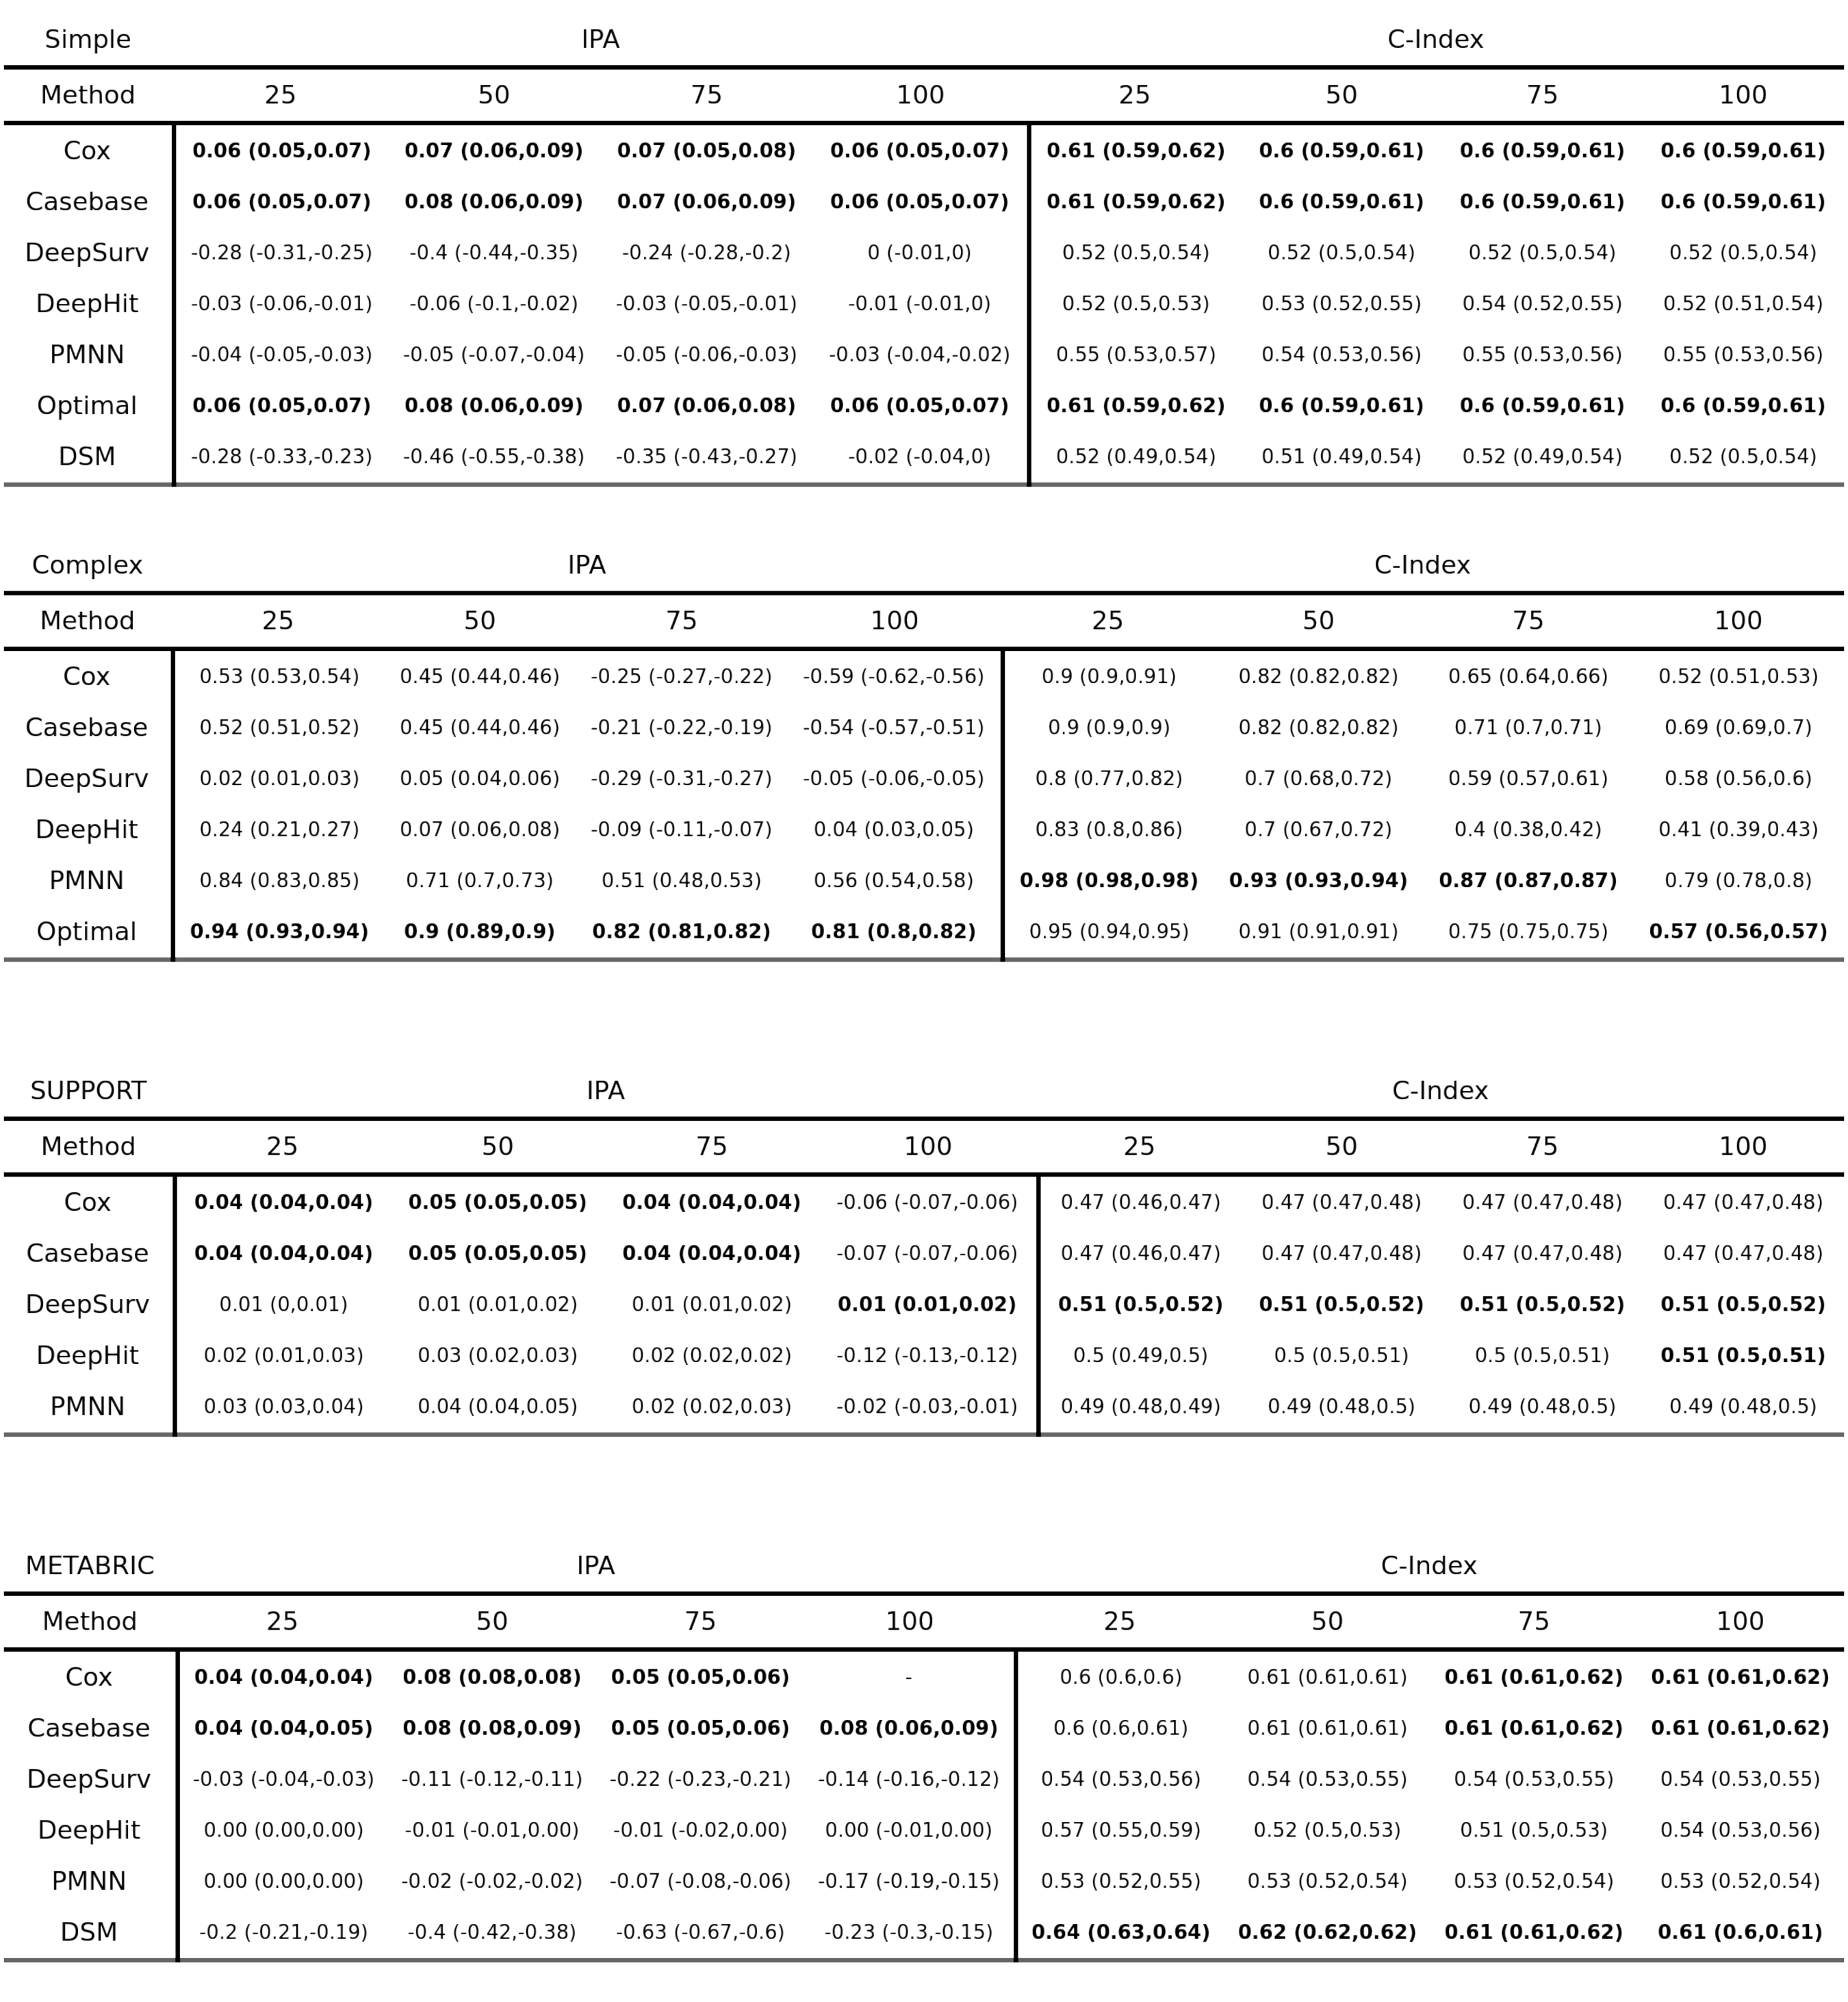
\includegraphics[width=1\linewidth]{/home/bhatnagar-lab/jislam/pmnnProjects/paper/../pmnnPlayground/reviewedAnalysisPMNN/figures/megaTable} \end{center}

\end{table}
\FloatBarrier

where
\(\gamma_{1}=3.9, \gamma_{2}=3, \gamma_{3}=-0.43, \gamma_{4}=1.33,\gamma_{5}=-0.86, \beta_{{1}}=1, \beta_{{2}}=1, \beta_{{3}}=1, \tau_{1}=10, \tau_{2}=2, \tau_{3}=2\)
and \(\psi\) are basis splines. To generate the \(gamma\) coefficients,
let \(g\): \(\mathbb{R} \rightarrow \mathbb{R}\) be a smoothing method
for variable \(t\) by a projection on to a set of basis functions on
splines:
\srb{i used gt as the function for splines. Specifically, natural cubic spline function of log time https://www.rdocumentation.org/packages/flexsurv/versions/2.1/topics/flexsurvspline . therefore, should i use g(log(t)) and and replace "smoothing method" with natural cubic spline? SAHIR: will fix any issues in this section in the final version.}
\begin{align}
g(t)=\sum^{m}_{l=1}\psi_{l} (t)\gamma_{l}.
\end{align}

An initial model with three knots (\(m=5\)) is fit using the
\emph{flexsurvspline} function with an intercept-only model on the data,
which returns the coefficients (\(\gamma\)) and basis of time (\(\psi\))
we use in our model. Note that we fix these values for the analysis. The
\(\beta\) coefficients represent direct effects, \(\tau_{2}\) and
\({\tau_3}\) represent interactions and \(\tau_{1}\) is a time-varying
interaction.

\hypertarget{performance-comparison-in-complex-simulation}{%
\subsubsection{Performance comparison in complex
simulation}\label{performance-comparison-in-complex-simulation}}

Figure \ref{fig:megaPlot} C, D and Table \ref{tab:megaTable} B show the
performance over time on a test set in the complex simulation. Apart
from the Optimal regression model, CBNN outperforms the competing models
when examining IPA, and up to the 75-percentile of follow-up time for
c-ipcw. We expected the Optimal model to perform best in both metrics.
However, this was not the case for c-ipcw and may be due to an artifact
of concordance-based metrics, where a misspecified model may perform
better than a correctly specified one \citep{cindexfails2019}. We
attribute this difference in performance to the flexibility of CBNN in
terms of time-varying interactions and baseline hazard, flexibility the
other neural network models do not have, explaining their drop in
performance.

\hypertarget{casestudies}{%
\section{Application to SUPPORT and METABRIC data}\label{casestudies}}

Our complex simulation demonstrates the superior performance of CBNN in
ideal conditions with clean data. To obtain a more realistic performance
assessment, we compared models using two real datasets with a
time-to-event outcome. The first case study examines the SUPPORT dataset
\citep{knaus1995SUPPORT}. The second case study examines the METABRIC
dataset \citep{curtis2012genomic}. We use the same hyperparameters as in
the simulation studies. As we do not know the true model for the real
data, we exclude the Optimal model. We split the datasets keeping 20\%
of the observations as a test set. 20\% of the training set is kept
aside for validation at each epoch. We predict risk functions for
everyone in the test set, which are used to calculate our metrics. We
conduct 100 bootstrap re-samples for the real data applications to
obtain confidence intervals.

\hypertarget{performance-evaluation-using-the-support-dataset}{%
\subsection{Performance evaluation using the SUPPORT
dataset}\label{performance-evaluation-using-the-support-dataset}}

The SUPPORT dataset tracks the time until death for seriously ill
patients at five American hospitals \citep{knaus1995SUPPORT}. We use a
pre-processed version of the dataset made available in the DeepSurv
package \citep{katzman2018DeepSurv}. This dataset contains 9104 samples
and 14 covariates (age, sex, race, number of comorbidities, presence of
diabetes, presence of dementia, presence of cancer, mean arterial blood
pressure, heart rate, respiration rate, temperature, white blood cell
count, serum's sodium, and serum's creatinine)
\citep{katzman2018DeepSurv}. Patients with missing features were
excluded and 68.10\% of the patients died during the 5.56-year study
period \citep{katzman2018DeepSurv}.

Figure \ref{fig:megaPlot} E, F and Table \ref{tab:megaTable} C
demonstrates the performance over time on a test set. The regression
models (CBLR, Cox) perform best considering IPA, followed by CBNN from
the \(25^{th}\) to \(100^{th}\) percentile of follow-up time. We note a
drop in performance for CBNN before the \(25^{th}\) percentile of
follow-up. For c-ipcw, CBNN outperforms the competing models
consistently over follow-up time. Note that performance is similar for
all models, aside from DeepSurv whose c-ipcw is lower than the rest
(Figure \ref{fig:megaPlot} E, F and Table \ref{tab:megaTable} C).

\hypertarget{performance-evaluation-using-the-metabric-dataset}{%
\subsection{Performance evaluation using the METABRIC
dataset}\label{performance-evaluation-using-the-metabric-dataset}}

METABRIC is a 30-yearlong study aiming to discover the molecular drivers
of breast tumors, following 2000 individuals with breast cancer until
death \citep{curtis2012genomic}. They described these growths as primary
invasive breast carcinomas, with the goal of discovering both genetic
and clinical risk factors for breast cancer survival
\citep{curtis2012genomic}. We used the processed dataset made available
through DeepSurv \citep{katzman2018DeepSurv}, which includes 1980
patients of which 57.72\% die due to breast cancer within a median 10
years of follow-up \citep{katzman2018DeepSurv}. There are 11 covariates
in total: 4 RNA-Seq gene expressions (MKI67, EGFR, PGR, and ERBB2) and 5
clinical features (hormone treatment indicator, radiotherapy indicator,
chemotherapy indicator, ER-positive indicator, and age at diagnosis)
\citep{katzman2018DeepSurv}.

Figure \ref{fig:megaPlot} G, H and Table \ref{tab:megaTable} D shows the
performance on a test set over time. The IPA scores suggest that
regression models outperform competing models on this dataset, as all
the neural network models are equal to or perform worse than KM over
follow-up time. Our CBNN model is comparable to KM until around the
50-percentile of follow-up time, after which CBNN, DeepSurv and DSM drop
in performance. The c-ipcw produces a different ranking. Our CBNN model
outperforms the other models up to the \(25^{th}\) percentile of
follow-up time, whereas DeepHit performs best from the \(50^{th}\) to
\(75^{th}\) percentile of follow-up. With this metric, CBNN and DeepHit
outperform the regression models. This disagreement between IPA and
c-ipcw between may be due to the misspecification issue of
concordance-based metrics \citep{cindexfails2019}. The neural network
models may be over-parameterized, as shown by the wide confidence bands
in c-ipcw.

\hypertarget{discussion}{%
\section{Discussion}\label{discussion}}

Our method, CBNN, models survival outcomes by using neural networks on
case-base sampled data. While estimating the hazard function, we
incorporate follow-up-time as a feature, providing a data-driven
estimation of a flexible baseline hazard and time-varying interactions.
Based on our complex simulation results (Figure \ref{fig:megaPlot} C, D
and Table \ref{tab:megaTable} B), CBNN outperforms the competitors when
time-varying interactions and a complex baseline hazard are present.

Each competing neural network model we evaluated has limitations or
model-specific parameters. DeepSurv is a proportional hazards model and
does not estimate the baseline hazard \citep{katzman2018DeepSurv}.
DeepHit requires an alpha hyperparameter, is restricted to a single
distribution for the baseline hazard, and models the survival function
directly \citep{lee2018DeepHit}. DSM requires the user to specify the
component distributions in the mixture for a flexible baseline hazard to
be fit \citep{dsmPaper}. These alternative neural network approaches
match on time, while CBNN models time directly.

In the simple simulation, all neural network-based approaches resulted
in a loss of performance based on IPA, while the regression-based
approaches did not. We attribute this to potential over-parameterization
in the neural network models. The wide confidence intervals suggest
over-fitting may be the reason for the loss in performance, even with
dropout. Both DeepSurv and DSM are affected, while DeepHit and CBNN are
less so.

In the complex simulation, CBNN has a distinct advantage over the other
methods while examining the IPA score. The regression models do show
improvement over the null model, while the competing neural network
approaches do not. The time-varying interactions and complex baseline
hazard may have caused a drop in performance for the competing neural
network methods, compared to the regression models without interactions.

In the SUPPORT application, the overall performance considering IPA is
near identical. The regression models outperform CBNN, which performs
better than the competing neural network models. As the confidence
intervals are tight, it is unlikely that the loss in performance is
because of over-fitting. Flexibility in both interaction modeling and
baseline hazard is not particularly helpful with the SUPPORT dataset.

In the METABRIC application IPA results, DSM and DeepSurv had a steep
drop in performance. As DeepSurv does not depend on the baseline hazard
during the fitting process and DSM is the most flexible competing model
in our comparison, the baseline hazard is unlikely to cause this drop.
With tight confidence intervals, over-fitting is unlikely as well.
Further research would be required to determine the cause of this drop
in performance. We do not see the same drop in CBNN demonstrating that,
in the METABRIC application, CBNN outperforms DeepSurv and DSM.
Considering IPA score, regression models consistently outperform the
neural network models. From a biological perspective, the 30-year
follow-up time in the METABRIC study may contain competing causes of
death. The signal from the start of the study may not match the signal
towards the end, potentially explaining the drop in performance as we
reach later survival times with fewer individuals.

Concordance-based measures are commonly used in survival analysis to
compare models and we opt to keep them in our analyses. However, c-ipcw
is a non-proper metric and may cause misspecified models to appear
better than they should \citep{cindexfails2019}. The model rankings
between c-ipcw and IPA differed for both the complex simulation and
METABRIC application. In the complex simulation, the c-ipcw of a
correctly specified model (Optimal) underperforms CBNN and CBLR; models
without the exact interaction terms specified. We base our METABRIC
assessment of this disagreement between metrics on the complex
simulation. The IPA score ranks regression models first, followed by
DeepHit and CBNN, but the c-ipcw score ranks regression models after
DeepHit and CBNN. Wide confidence intervals for neural network models in
c-ipcw show potential misspecification, suggesting that regression
models perform best in the METABRIC application.

During our testing for the complex simulation and SUPPORT application,
DSM did not converge with our choice of hyper-parameters and model
design. As the goal is to fix the design and compare performance, we did
not change any shared hyperparameters. For DSM, a different number and
combination of component distributions did not help the model converge,
though we did not conduct an exhaustive test. This may be a limitation
to their method or early-stage implementation issues. We include this
method where it did function as it shares a similar goal of a flexible
baseline hazard.

If the user suspects that there may be unknown time-varying interactions
and a complex baseline hazard, CBNN should strongly be considered. Once
we perform case-base sampling and adjust for the sampling bias, we can
use a sigmoid activation function to predict our hazard function. The
user can approach their problem as they would for probabilistic modeling
while interpreting their prediction in a survival context. In terms of
performance, we saw that CBNN consistently performs better than the
other neural network-based approaches over follow-up time. This may be
because of the hyperparameters chosen, as they differ from each of the
respective methods papers. CBNN only requires the use of standard
components in machine learning libraries (add layer and sigmoid
activation function). Due to the simplicity in its implementation and by
extension user experience, we expect CBNN to be both a user-friendly
approach to data-driven survival analysis and easily extendable to any
feed-forward neural network frameworks.

Though CBNN can model time-varying interactions and a flexible baseline
hazard, all models require substantial amounts of data to learn real,
complex relationships effectively. Larger datasets will appear with
time, but the cost of generating longitudinal datasets remains. A viable
alternative strategy is the use of transfer learning, where independent
and identically distributed data can function as a preliminary model to
learn related features in a parallel dataset, initializing weights for
our survival task \citep{bozinovski2020reminder}.

This paper describes CBNN in the single event setting. A next step would
be to extend this approach to competing risks. A promising use case
would be high-dimensional data with complex correlation structures, such
as imaging data.

\bibliography{bibfile.bib}


\end{document}
